% Options for packages loaded elsewhere
\PassOptionsToPackage{unicode}{hyperref}
\PassOptionsToPackage{hyphens}{url}
\PassOptionsToPackage{dvipsnames,svgnames,x11names}{xcolor}
%
\documentclass[
  letterpaper,
  DIV=11,
  numbers=noendperiod]{scrartcl}

\usepackage{amsmath,amssymb}
\usepackage{iftex}
\ifPDFTeX
  \usepackage[T1]{fontenc}
  \usepackage[utf8]{inputenc}
  \usepackage{textcomp} % provide euro and other symbols
\else % if luatex or xetex
  \usepackage{unicode-math}
  \defaultfontfeatures{Scale=MatchLowercase}
  \defaultfontfeatures[\rmfamily]{Ligatures=TeX,Scale=1}
\fi
\usepackage{lmodern}
\ifPDFTeX\else  
    % xetex/luatex font selection
\fi
% Use upquote if available, for straight quotes in verbatim environments
\IfFileExists{upquote.sty}{\usepackage{upquote}}{}
\IfFileExists{microtype.sty}{% use microtype if available
  \usepackage[]{microtype}
  \UseMicrotypeSet[protrusion]{basicmath} % disable protrusion for tt fonts
}{}
\makeatletter
\@ifundefined{KOMAClassName}{% if non-KOMA class
  \IfFileExists{parskip.sty}{%
    \usepackage{parskip}
  }{% else
    \setlength{\parindent}{0pt}
    \setlength{\parskip}{6pt plus 2pt minus 1pt}}
}{% if KOMA class
  \KOMAoptions{parskip=half}}
\makeatother
\usepackage{xcolor}
\setlength{\emergencystretch}{3em} % prevent overfull lines
\setcounter{secnumdepth}{5}
% Make \paragraph and \subparagraph free-standing
\ifx\paragraph\undefined\else
  \let\oldparagraph\paragraph
  \renewcommand{\paragraph}[1]{\oldparagraph{#1}\mbox{}}
\fi
\ifx\subparagraph\undefined\else
  \let\oldsubparagraph\subparagraph
  \renewcommand{\subparagraph}[1]{\oldsubparagraph{#1}\mbox{}}
\fi


\providecommand{\tightlist}{%
  \setlength{\itemsep}{0pt}\setlength{\parskip}{0pt}}\usepackage{longtable,booktabs,array}
\usepackage{calc} % for calculating minipage widths
% Correct order of tables after \paragraph or \subparagraph
\usepackage{etoolbox}
\makeatletter
\patchcmd\longtable{\par}{\if@noskipsec\mbox{}\fi\par}{}{}
\makeatother
% Allow footnotes in longtable head/foot
\IfFileExists{footnotehyper.sty}{\usepackage{footnotehyper}}{\usepackage{footnote}}
\makesavenoteenv{longtable}
\usepackage{graphicx}
\makeatletter
\def\maxwidth{\ifdim\Gin@nat@width>\linewidth\linewidth\else\Gin@nat@width\fi}
\def\maxheight{\ifdim\Gin@nat@height>\textheight\textheight\else\Gin@nat@height\fi}
\makeatother
% Scale images if necessary, so that they will not overflow the page
% margins by default, and it is still possible to overwrite the defaults
% using explicit options in \includegraphics[width, height, ...]{}
\setkeys{Gin}{width=\maxwidth,height=\maxheight,keepaspectratio}
% Set default figure placement to htbp
\makeatletter
\def\fps@figure{htbp}
\makeatother
\newlength{\cslhangindent}
\setlength{\cslhangindent}{1.5em}
\newlength{\csllabelwidth}
\setlength{\csllabelwidth}{3em}
\newlength{\cslentryspacingunit} % times entry-spacing
\setlength{\cslentryspacingunit}{\parskip}
\newenvironment{CSLReferences}[2] % #1 hanging-ident, #2 entry spacing
 {% don't indent paragraphs
  \setlength{\parindent}{0pt}
  % turn on hanging indent if param 1 is 1
  \ifodd #1
  \let\oldpar\par
  \def\par{\hangindent=\cslhangindent\oldpar}
  \fi
  % set entry spacing
  \setlength{\parskip}{#2\cslentryspacingunit}
 }%
 {}
\usepackage{calc}
\newcommand{\CSLBlock}[1]{#1\hfill\break}
\newcommand{\CSLLeftMargin}[1]{\parbox[t]{\csllabelwidth}{#1}}
\newcommand{\CSLRightInline}[1]{\parbox[t]{\linewidth - \csllabelwidth}{#1}\break}
\newcommand{\CSLIndent}[1]{\hspace{\cslhangindent}#1}

\usepackage{booktabs}
\usepackage{longtable}
\usepackage{array}
\usepackage{multirow}
\usepackage{wrapfig}
\usepackage{float}
\usepackage{colortbl}
\usepackage{pdflscape}
\usepackage{tabu}
\usepackage{threeparttable}
\usepackage{threeparttablex}
\usepackage[normalem]{ulem}
\usepackage{makecell}
\usepackage{xcolor}
\KOMAoption{captions}{tableheading}
\makeatletter
\makeatother
\makeatletter
\makeatother
\makeatletter
\@ifpackageloaded{caption}{}{\usepackage{caption}}
\AtBeginDocument{%
\ifdefined\contentsname
  \renewcommand*\contentsname{Table of contents}
\else
  \newcommand\contentsname{Table of contents}
\fi
\ifdefined\listfigurename
  \renewcommand*\listfigurename{List of Figures}
\else
  \newcommand\listfigurename{List of Figures}
\fi
\ifdefined\listtablename
  \renewcommand*\listtablename{List of Tables}
\else
  \newcommand\listtablename{List of Tables}
\fi
\ifdefined\figurename
  \renewcommand*\figurename{Figure}
\else
  \newcommand\figurename{Figure}
\fi
\ifdefined\tablename
  \renewcommand*\tablename{Table}
\else
  \newcommand\tablename{Table}
\fi
}
\@ifpackageloaded{float}{}{\usepackage{float}}
\floatstyle{ruled}
\@ifundefined{c@chapter}{\newfloat{codelisting}{h}{lop}}{\newfloat{codelisting}{h}{lop}[chapter]}
\floatname{codelisting}{Listing}
\newcommand*\listoflistings{\listof{codelisting}{List of Listings}}
\makeatother
\makeatletter
\@ifpackageloaded{caption}{}{\usepackage{caption}}
\@ifpackageloaded{subcaption}{}{\usepackage{subcaption}}
\makeatother
\makeatletter
\@ifpackageloaded{tcolorbox}{}{\usepackage[skins,breakable]{tcolorbox}}
\makeatother
\makeatletter
\@ifundefined{shadecolor}{\definecolor{shadecolor}{rgb}{.97, .97, .97}}
\makeatother
\makeatletter
\makeatother
\makeatletter
\makeatother
\ifLuaTeX
  \usepackage{selnolig}  % disable illegal ligatures
\fi
\IfFileExists{bookmark.sty}{\usepackage{bookmark}}{\usepackage{hyperref}}
\IfFileExists{xurl.sty}{\usepackage{xurl}}{} % add URL line breaks if available
\urlstyle{same} % disable monospaced font for URLs
\hypersetup{
  pdftitle={Structural Insights 2023: A Linear Analysis of Apartment Age and Safety Scores in Toronto},
  pdfauthor={Terry Tu, Jingyi Shen, Yaning Jin},
  colorlinks=true,
  linkcolor={blue},
  filecolor={Maroon},
  citecolor={Blue},
  urlcolor={Blue},
  pdfcreator={LaTeX via pandoc}}

\title{Structural Insights 2023: A Linear Analysis of Apartment Age and
Safety Scores in Toronto\thanks{Code and data supporting this analysis
are available at
https://github.com/TEJMaster/Toronto-Building-Safety-Analysis-2023.git}}
\author{Terry Tu, Jingyi Shen, Yaning Jin}
\date{March 15, 2024}

\begin{document}
\maketitle
\begin{abstract}
This study harnesses a dataset from the Toronto Open Data portal,
comprising 3,435 records of apartment evaluations, to analyze the
correlation between building age and safety scores. Employing a linear
regression model, we discovered a significant inverse relationship,
highlighting that older buildings tend to have lower safety evaluations.
The findings suggest a need for policy reform, particularly in the
maintenance and inspection of Toronto's aging residential
infrastructure. Despite the study's focus on building age, further
research considering additional variables could offer a more
comprehensive understanding of factors influencing building safety.
\end{abstract}
\ifdefined\Shaded\renewenvironment{Shaded}{\begin{tcolorbox}[borderline west={3pt}{0pt}{shadecolor}, sharp corners, interior hidden, breakable, frame hidden, boxrule=0pt, enhanced]}{\end{tcolorbox}}\fi

\renewcommand*\contentsname{Table of contents}
{
\hypersetup{linkcolor=}
\setcounter{tocdepth}{1}
\tableofcontents
}
\hypertarget{introduction}{%
\section{Introduction}\label{introduction}}

The structural integrity of urban buildings is a paramount concern for
city planners, policymakers, and residents alike. The tragic collapse of
a condominium in South Florida in June 2021, which resulted in 98
casualties, serves as a stark reminder of the potential consequences of
neglecting building maintenance and inspections
(\protect\hyperlink{ref-Anderson_2021}{Anderson 2021}). This event
highlights a critical gap in our understanding of the factors that
contribute to the safety and longevity of urban residential structures.
In light of this, our study aims to investigate the relationship between
building age and evaluation scores in the context of Toronto's
residential buildings.

Our study's estimand is the effect of building age on evaluation scores
in Toronto. We investigate how the age of buildings influences their
assigned evaluation scores, reflecting their compliance with safety
standards and overall condition. Utilizing a dataset from the Toronto
Open Data portal, which includes 3,435 records, we apply a simple linear
regression model to forecast evaluation scores for Toronto residences in
2023. By conducting this analysis, we aim to quantify the impact of
building age on evaluation scores and understand its implications for
urban housing safety and maintenance.

The analysis reveals a statistically significant inverse relationship
between building age and evaluation score, indicating that older
buildings tend to receive lower evaluation scores. This finding
highlights the critical need for regular inspections and maintenance to
preserve the safety and habitability of aging buildings. It also
suggests that policies should prioritize the maintenance and inspection
of older structures to prevent potential safety hazards.

Moreover, our study offers insights into urban development and
maintenance, suggesting that policymakers might need to revisit
regulations surrounding building inspections and maintenance schedules.
It further emphasizes the importance of continuous monitoring and
evaluation by urban authorities to maintain and enhance housing
standards across the city. These insights carry substantial implications
for urban planning and public safety, underscoring the necessity of
proactive measures to mitigate risks associated with aging
infrastructure. In conclusion, this paper significantly advances our
understanding of the relationship between building age and evaluation
scores, underlining the importance of proactive strategies to ensure the
safety and integrity of the urban housing stock.

The remainder of this paper is structured as follows:
Section~\ref{sec-data} (Data) details the raw data, the cleaning
process, and provides an overview of the data distribution.
Section~\ref{sec-model} (Model) describes the linear model employed to
predict the building evaluation score based on the building's age.
Section~\ref{sec-result} (Results) presents the coefficients of the
linear model, analyses the residuals, and includes a plot illustrating
the linear model applied to the analysis dataset. Finally,
Section~\ref{sec-discussion} (Discussion) discusses the limitations of
the analysis and suggests potential insights for future research.

\hypertarget{sec-data}{%
\section{Data}\label{sec-data}}

\hypertarget{raw-data}{%
\subsection{Raw Data}\label{raw-data}}

In this research, we examine apartment data sourced using the
\texttt{opendatatoronto} package
(\protect\hyperlink{ref-Toronto_2023}{Toronto 2023}). The dataset
encompasses 3,435 records, focusing on specific variables: the ward of
each apartment, its evaluation score, and the construction year. The
data covers evaluations across Toronto's 25 wards, with scores varying
between a minimum of 0 and some achieving the maximum score of 100. The
study includes apartments that are over three stories in height and
contain at least 10 units. These apartments span a wide range of
construction years, from as early as 1805 to as recent as 2023. All the
apartments in this dataset adhere to the City's Apartment Building
Standards bylaw, which is designed to safeguard the interests and safety
of both landlords and tenants by mandating these evaluations.

\hypertarget{data-analysis-tools}{%
\subsection{Data Analysis Tools}\label{data-analysis-tools}}

The data analysis was performed using R (\protect\hyperlink{ref-r}{R
Core Team 2022}), a powerful open-source statistical programming
language. A suite of packages from the tidyverse
(\protect\hyperlink{ref-rTidyverse}{Wickham et al. 2019}), an assemblage
of R packages designed for data science, was harnessed to enhance the
efficiency of our data operations. The \texttt{ggplot2} package
(\protect\hyperlink{ref-rGgplot2}{Wickham 2016}) facilitated the
creation of sophisticated visualizations, while \texttt{dplyr}
(\protect\hyperlink{ref-rDplyr}{Wickham et al. 2022}) provided a grammar
of data manipulation, offering a coherent set of verbs that help in
filtering, summarizing, and arranging the dataset. The \texttt{readr}
package (\protect\hyperlink{ref-rReadr}{Wickham, Hester, and Bryan
2022}) was utilized for its fast and friendly data reading capabilities.
Navigation and file path management were streamlined using the
\texttt{here} package (\protect\hyperlink{ref-R-here}{Müller 2020}),
simplifying the process of file referencing within the project's
directory structure. Report generation was dynamically handled by knitr
(\protect\hyperlink{ref-rKnitr}{Xie 2014}), enabling the integration of
R code within this document. Additionally,
\texttt{kableExtra}(\protect\hyperlink{ref-R-kableExtra}{Zhu 2021}) was
employed to produce aesthetically pleasing and customizable tables,
enriching the presentation of our results. For the Bayesian analysis,
rstanarm (\protect\hyperlink{ref-R-rstanarm}{Goodrich et al. 2020}) was
utilized to create a linear model, providing an elegant interface to
Stan, a state-of-the-art platform for statistical modeling and
high-performance statistical computation. This package enabled us to
estimate the relationship between building age and safety evaluation
scores using a Bayesian framework.

\hypertarget{variable-description}{%
\subsection{Variable Description}\label{variable-description}}

CURRENT BUILDING EVAL SCORE: The Current Building Evaluation Score
represents a measure of a building's adherence to property standards.
This score is derived by summing two components: the current reactive
score, which reflects the compliance based on any outstanding Orders and
Notices of Violations, and the proactive building score, which is based
on the most recent comprehensive evaluation of the building.

YEAR BUILT: This indicates the year when the building was initially
constructed, sourced from Building Owners/Managers.

YEAR EVALUATED: This denotes the year in which the building underwent
evaluation, reflecting its condition and performance.

AGE: In this research, neither YEAR BUILT nor YEAR EVALUATED was used
directly, we have generated a new variable called AGE which use YEAR
EVALUATED minus YEAR BUILT.

\hypertarget{sample-of-cleaned-building-evaluation-data}{%
\subsection{Sample of Cleaned Building Evaluation
Data}\label{sample-of-cleaned-building-evaluation-data}}

\hypertarget{tbl-data-sample}{}
\begin{longtable}[]{@{}rrr@{}}
\caption{\label{tbl-data-sample}Sample of Building Evaluation
Data}\tabularnewline
\toprule\noalign{}
Building ID & Age (Years) & Evaluation Score \\
\midrule\noalign{}
\endfirsthead
\toprule\noalign{}
Building ID & Age (Years) & Evaluation Score \\
\midrule\noalign{}
\endhead
\bottomrule\noalign{}
\endlastfoot
1 & 62 & 86 \\
2 & 44 & 94 \\
3 & 54 & 78 \\
4 & 73 & 89 \\
5 & 54 & 99 \\
6 & 53 & 99 \\
\end{longtable}

Table~\ref{tbl-data-sample} represents a subset of the larger building
evaluation data. Each row corresponds to a unique building identified by
X\_id. The AGE column indicates the age of the building in years, while
the CURRENT.BUILDING.EVAL.SCORE column shows the building's current
evaluation score on a scale from 0 to 100, with higher scores indicating
better compliance with safety standards.

\hypertarget{measurement}{%
\subsection{Measurement:}\label{measurement}}

\newpage

\hypertarget{data-exploration}{%
\subsection{Data Exploration:}\label{data-exploration}}

\hypertarget{data-summary}{%
\subsubsection{Data Summary}\label{data-summary}}

\hypertarget{tbl-summary-table}{}
\begin{longtable}[t]{>{}ccccc}
\caption{\label{tbl-summary-table}Summary Statistics for the Cleaned Dataset }\tabularnewline

\toprule
Count & Mean Age (Years) & SD of Age (Years) & Mean Score & SD of Score\\
\midrule
\textbf{1748} & 60.644 & 19.939 & 87.504 & 8.693\\
\bottomrule
\end{longtable}

Table~\ref{tbl-summary-table} presents a concise overview of the key
descriptive metrics for the age of buildings and their evaluation scores
within the dataset:

\begin{itemize}
\item
  \textbf{Count}: The dataset encompasses a total of 1,748 buildings,
  indicating a robust sample size for statistical analysis.
\item
  \textbf{Mean Age}: The average age of the buildings is approximately
  60.644 years, suggesting that the dataset primarily includes buildings
  that have been standing for over half a century.
\item
  \textbf{Standard Deviation of Age}: With a standard deviation of about
  19.939 years, there is considerable variability in the ages of the
  buildings. This range implies a diverse sample, encompassing both
  relatively new constructions and much older structures.
\item
  \textbf{Mean Score}: The average building evaluation score is
  approximately 87.504 on a scale from 0 to 100. A higher score
  corresponds to better adherence to safety and maintenance standards,
  suggesting that the buildings in this dataset are generally
  well-maintained.
\item
  \textbf{Standard Deviation of Score}: The standard deviation of
  approximately 8.693 for the evaluation scores indicates that while
  scores are clustered around a high mean, there is still notable
  variability, reflecting differences in the condition or compliance of
  the buildings.
\end{itemize}

These statistics offer a snapshot of the dataset's characteristics,
providing foundational insights for further analysis regarding the state
of building safety and integrity in the population studied.

\hypertarget{age-distribution}{%
\subsubsection{Age Distribution}\label{age-distribution}}

\begin{figure}

{\centering 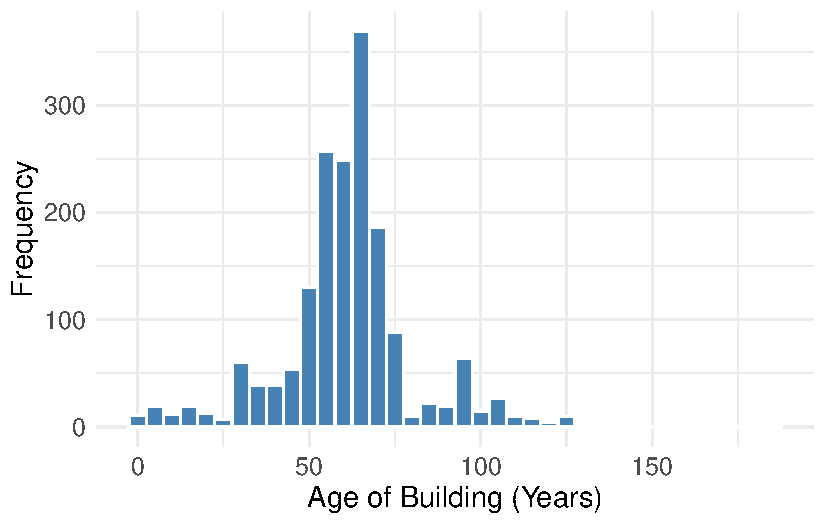
\includegraphics{paper_files/figure-pdf/fig-age-distribution-1.pdf}

}

\caption{\label{fig-age-distribution}Distribution of building's age for
the cleaned data set}

\end{figure}

Figure~\ref{fig-age-distribution} illustrates the frequency distribution
of the ages of buildings within the dataset. The x-axis represents the
age of the buildings in years, while the y-axis shows the frequency of
buildings within each age range. The distribution appears to be unimodal
with a peak around the 50-year mark, indicating that a substantial
number of the buildings within this dataset were constructed around half
a century ago. Following this peak, the frequency gradually decreases,
showing that fewer buildings have been in existence beyond this age. The
distribution suggests a relatively young building population, with ages
concentrated below 100 years, and very few buildings reaching beyond 120
years of age. This visualization aids in understanding the age profile
of buildings under consideration for safety evaluation scoring.

\hypertarget{score-distribution}{%
\subsubsection{Score Distribution}\label{score-distribution}}

\begin{figure}

{\centering 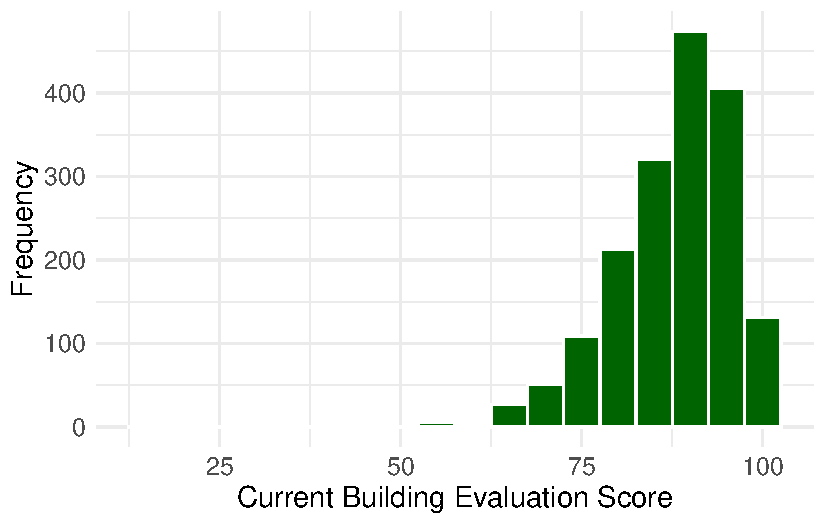
\includegraphics{paper_files/figure-pdf/fig-score-distribution-1.pdf}

}

\caption{\label{fig-score-distribution}Distribution of building's
evaluation score for the cleaned data set}

\end{figure}

Figure~\ref{fig-score-distribution} showcases the distribution of
building evaluation scores. The x-axis represents the scores assigned to
buildings, which can range from 0 to 100, with the y-axis displaying the
frequency of buildings for each score interval. The chart reveals a
concentration of high evaluation scores, suggesting that many of the
buildings in the dataset are rated as being in good or excellent
condition according to the evaluation criteria. The tallest bars are
clustered towards the higher end of the score range, indicating that
buildings with scores close to 100 are prevalent. This positive skew in
the distribution might reflect effective building standards and
maintenance practices in place. The spread of the scores and their
frequency can offer insights into the overall health of the evaluated
buildings, influencing urban planning and policy development.

\hypertarget{sec-model}{%
\section{Model}\label{sec-model}}

The objective of our model is dual: to discern the relationship between
building age and safety evaluation scores and to quantify this
relationship's strength and direction. The study utilizes a simple
linear regression model to analyze the dataset obtained from the Toronto
Open Data portal.

\hypertarget{model-set-up}{%
\subsection{Model set-up}\label{model-set-up}}

Let \(y_i\) represent the safety evaluation score for each building. The
building's age is denoted by \(x_i\).The model is defined as follows:

\begin{align}
y_i &\sim \mbox{Normal}(\mu_i, \sigma) \\
\mu_i &= \beta_0 + \beta_1 \times \mbox{AGE}_i \\
\beta_0 &\sim \mbox{Normal}(85, 10) \\
\beta_1 &\sim \mbox{Normal}(0, 0.05)
\end{align}

The model is implemented in R using the rstanarm package, which allows
us to incorporate prior beliefs about the parameters and to estimate the
posterior distributions. For the intercept \(\beta_0\) and slope
\(\beta_1\) , we choose normal prior distributions centered around our
initial estimates based on exploratory data analysis. The
\texttt{stan\_glm} function from \texttt{rstanarm} is utilized to carry
out the Bayesian regression, providing a framework for inference that
incorporates both the data and our prior knowledge.

The priors are chosen to reflect reasonable beliefs about the parameters
before observing the data. The intercept prior reflects an expectation
that a new building will have a high safety score around 90, with a wide
spread to accommodate uncertainty. Similarly, the slope prior indicates
an expected small negative impact of age on the safety score,
acknowledging some uncertainty in the precise effect. The
\texttt{stan\_glm} function combines these priors with the data to
estimate the posterior distributions of the model parameters.

\hypertarget{model-justification}{%
\subsection{Model justification}\label{model-justification}}

We hypothesize that the coefficient for building age (\(\beta_1\)) will
be negative, reflecting the tendency for older buildings to exhibit
lower safety scores. This expectation is rooted in the general
understanding that buildings can deteriorate over time due to wear,
aging materials, and possible obsolescence in older construction
methods. The intercept (\(\beta_0\)), representing the baseline
evaluation score for a new building, is presumed to be relatively high,
indicating the score a building would receive if it were built in the
current period with modern standards. The slope (\(\beta_1\)) is
therefore of particular interest, as it encapsulates the average annual
decline in evaluation score attributable to aging. The Bayesian
framework allows us to incorporate these hypotheses as priors in our
model, thereby aligning the analysis with our substantive expectations
and providing a more nuanced interpretation of the data.

\hypertarget{sec-result}{%
\section{Result}\label{sec-result}}

\hypertarget{model-coefficients-interpretation}{%
\subsection{Model Coefficients
Interpretation}\label{model-coefficients-interpretation}}

\hypertarget{tbl-coefficient-table}{}
\begin{longtable}[t]{cc}
\caption{\label{tbl-coefficient-table}Summary Statistics for the Coefficients of the Linear Model }\tabularnewline

\toprule
Term & Estimate\\
\midrule
Intercept & 93.364\\
Slope & -0.097\\
\bottomrule
\end{longtable}

Table~\ref{tbl-coefficient-table} provides two key coefficients to
understand the relationship between building age and the evaluation
score:

\textbf{Intercept} (\(\beta_0\)):\\
The model's intercept, \(\beta_0\), has an estimate of 93.364. This
represents the baseline evaluation score for a hypothetical newly
constructed building. The intercept suggests that if a building were
constructed in the current year, its expected evaluation score would be
around 93.364, assuming all other factors remain constant.

\textbf{Slope} (\(\beta_1\)):\\
The slope parameter, \(\beta_1\), has an estimate of -0.097. This
indicates that, on average, the evaluation score is expected to decrease
by approximately 0.097 points for each additional year of a building's
age. This negative value suggests a trend where older buildings tend to
have lower evaluation scores compared to newer ones.

\textbf{Interpretation}: The analysis suggests a negative relationship
between building age and evaluation score. The estimates indicate that
newer buildings tend to have higher evaluation scores, which decrease as
buildings age. This trend highlights the importance of age as a factor
in building evaluations and underscores the need for ongoing maintenance
and updates to preserve building safety and integrity over time.

\hypertarget{model-equation}{%
\subsection{Model Equation}\label{model-equation}}

\begin{align}
y_i &\sim \mbox{Normal}(\mu_i, \sigma) \\
\mu_i &= \beta_0 + \beta_1 \times x_i \\
\beta_0 &= 93.364 \\
\beta_1 &= -0.097
\end{align}

In this model, \(y_i\) represents the predicted evaluation score for the
\(i\)-th building, \(x_i\) represents the age for the \(i\)-th building,
\(\mu_i\) is the mean of the normal distribution for the \(i\)-th
observation, \(\beta_0\) is the intercept, and \(\beta_1\) is the slope
representing the change in evaluation score per year of building age.

\hypertarget{analysis-of-residuals}{%
\subsection{Analysis of Residuals}\label{analysis-of-residuals}}

\hypertarget{tbl-residuals-summary}{}
\begin{longtable}[]{@{}cc@{}}
\caption{\label{tbl-residuals-summary}Summary Statistics for the
Residuals of the Bayesian Linear Model}\tabularnewline
\toprule\noalign{}
Residual Statistics & Value \\
\midrule\noalign{}
\endfirsthead
\toprule\noalign{}
Residual Statistics & Value \\
\midrule\noalign{}
\endhead
\bottomrule\noalign{}
\endlastfoot
Min & -69.700 \\
1st Qu. & -4.440 \\
Median & 1.687 \\
Mean & -0.003 \\
3rd Qu. & 5.860 \\
Max & 15.715 \\
\end{longtable}

\textbf{1. Minimum Residual}: The minimum residual is -69.700,
indicating that there is at least one building for which the model's
predicted evaluation score was lower than the actual score by
approximately 69.700 points. This could be an outlier or a building with
exceptional characteristics not captured by the model.

\textbf{2. First Quartile Residual}: The first quartile (Q1) of the
residuals is -4.440, meaning that 25\% of the buildings have evaluation
scores that are less than 4.440 points below the model's prediction for
their age.

\textbf{3. Median Residual}: The median residual is 1.687, suggesting a
slight positive bias in the model's predictions, as the median of the
error distribution is above zero. This indicates that, on average, the
model tends to slightly overestimate the evaluation scores.

\textbf{4. Third Quartile Residual}: The third quartile (Q3) is 5.860,
indicating that 75\% of the buildings have evaluation scores within
5.860 points of the model's predictions or better. This shows that the
model provides reasonably accurate predictions for the majority of
buildings.

\textbf{5. Maximum Residual}: The maximum residual is 15.715, suggesting
that there is at least one building for which the model's predicted
evaluation score was higher than the actual score by approximately
15.715 points. This could be another outlier or a building that
performed exceptionally well.

\textbf{Interpretation}: The residuals provide insights into the model's
fit and the distribution of errors. The presence of outliers and the
distribution's slight asymmetry warrant further investigation. It's
crucial to assess the model's assumptions, such as linearity,
homoscedasticity, and normality of residuals, to ensure the validity of
the statistical inferences made from the model. Understanding the
reasons behind significant deviations can help improve the model and
provide more accurate predictions.

\hypertarget{plot-for-the-linear-model}{%
\subsection{Plot for the linear model}\label{plot-for-the-linear-model}}

\begin{figure}

{\centering 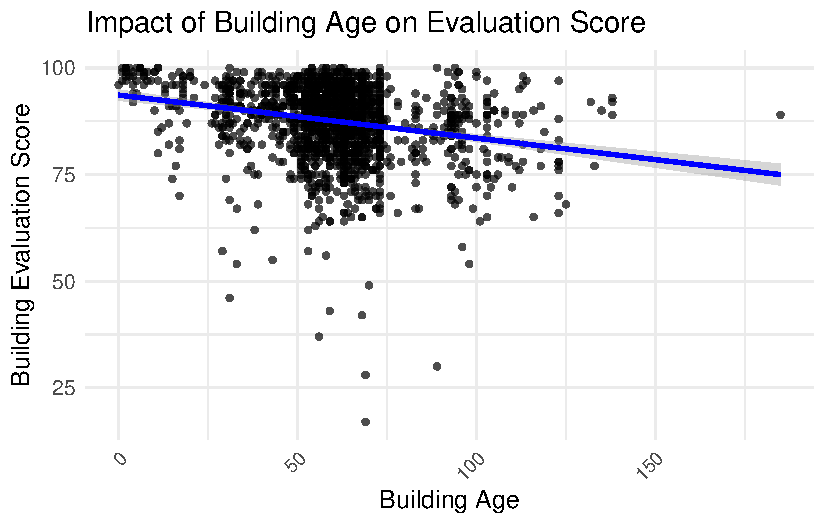
\includegraphics{paper_files/figure-pdf/fig-linear-plot-1.pdf}

}

\caption{\label{fig-linear-plot}plot for the linear relationship between
building age and evaluation score}

\end{figure}

Figure~\ref{fig-linear-plot} provides a clear visual relationship
between the age of buildings and their evaluation scores. Displayed with
building age on the x-axis and evaluation score on the y-axis, the data
points represent individual apartment buildings. The blue line running
through the cluster of points represents the linear regression line,
which captures the average effect of age on evaluation score.
Noticeably, the slope of the line is downward, suggesting a negative
correlation; as the buildings get older, their evaluation scores tend to
decrease. This trend is consistent across the dataset, indicating a
general decline in scores as building age increases, a reflection of the
typical effects of wear and time on building integrity.

The plot also reveals that while younger buildings cluster more densely
around higher evaluation scores, older buildings exhibit a wider spread
of scores. This variation suggests that other factors may influence the
condition and safety of older buildings, which are not captured solely
by age. The plot does not show any clear pattern or funnel shape in the
residuals, indicating that the variance of the evaluation scores is
fairly consistent across the range of building ages, and the assumption
of homoscedasticity is not visibly violated. Nonetheless, the model's
findings imply the importance of consistent maintenance and updates to
older buildings to ensure safety standards are upheld over time.

\hypertarget{sec-discussion}{%
\section{Discussion}\label{sec-discussion}}

\hypertarget{overview-of-the-study}{%
\subsection{Overview of the Study}\label{overview-of-the-study}}

This paper presented a detailed analysis using simple linear regression
to investigate the impact of building age on the evaluation scores
assigned by the City of Toronto. By analyzing data from the Toronto Open
Data portal, the study aimed to forecast evaluation scores for Toronto
residences in 2023. The analysis revealed a statistically significant
inverse relationship between building age and evaluation score,
suggesting that older buildings tend to have lower evaluation scores.

\hypertarget{insights-into-urban-development-and-maintenance}{%
\subsection{Insights into Urban Development and
Maintenance}\label{insights-into-urban-development-and-maintenance}}

One key insight from this study is the importance of building age in the
overall health and safety of urban residential environments. The
findings underscore the potential risks associated with older buildings,
which may not meet modern standards or may have deteriorated over time.
This knowledge emphasizes the need for regular inspections, maintenance,
and upgrades to older buildings to ensure they remain safe and
habitable. Additionally, the study highlights the value of continuous
monitoring and evaluation by urban authorities to maintain and improve
housing standards across the city.

\hypertarget{policy-implications-and-housing-quality}{%
\subsection{Policy Implications and Housing
Quality}\label{policy-implications-and-housing-quality}}

Another significant insight relates to the policy implications for
housing quality and safety standards. The correlation between building
age and lower evaluation scores may prompt policymakers to reconsider
regulations surrounding building inspections, maintenance schedules, and
renovation requirements. It suggests an opportunity for targeted
interventions in older buildings to prevent potential hazards and
improve living conditions for residents. Moreover, these findings could
guide urban planning strategies, prioritizing the revitalization of
aging housing stock and ensuring equitable access to safe and quality
housing.

\hypertarget{limitations-of-the-study}{%
\subsection{Limitations of the Study}\label{limitations-of-the-study}}

Despite its contributions, this study has several limitations. Firstly,
the model accounts for only a small fraction of the variability in
evaluation scores, indicating that other factors besides building age
significantly influence these scores. The exclusion of variables such as
building materials, design, maintenance history, and location may limit
the comprehensiveness of the findings. Additionally, the model's
assumptions (e.g., linearity and homoscedasticity) and the presence of
outliers suggest caution in generalizing the results without further
investigation.

\hypertarget{future-directions}{%
\subsection{Future Directions}\label{future-directions}}

Given the limitations and the insights gained, future research should
aim to incorporate additional variables that could affect building
evaluation scores. A more comprehensive model including factors like
renovation history, compliance with current building codes, and
socio-economic characteristics of the neighborhood could provide a
deeper understanding of what influences building evaluation scores.
Longitudinal studies could also shed light on the trends over time,
offering insights into the effectiveness of policy interventions and
maintenance practices. Moreover, comparative analyses across different
cities or countries could highlight unique challenges and best practices
in building maintenance and safety standards.

In conclusion, while this study has provided valuable insights into the
impact of building age on evaluation scores, it also opens the door for
further research to explore the multifaceted nature of building quality
and safety. Addressing these questions is crucial for developing
effective strategies to improve urban living conditions and ensure the
longevity and safety of the housing stock.

\hypertarget{appendix}{%
\section{Appendix}\label{appendix}}

\hypertarget{references}{%
\section*{References}\label{references}}
\addcontentsline{toc}{section}{References}

\hypertarget{refs}{}
\begin{CSLReferences}{1}{0}
\leavevmode\vadjust pre{\hypertarget{ref-Anderson_2021}{}}%
Anderson, Curt. 2021. {``Lawsuit Claims Surfside Condo Collapse
Triggered by Building Work.''} \emph{NBC 6 South Florida}. NBC 6 South
Florida.
\href{http://www.nbcmiami.com/news/local/lawsuit-claims-surfside-condo-collapse-triggered-by-building-w\%20ork/2622574/.}{http://www.nbcmiami.com/news/local/lawsuit-claims-surfside-condo-collapse-triggered-by-building-w
ork/2622574/.}

\leavevmode\vadjust pre{\hypertarget{ref-R-rstanarm}{}}%
Goodrich, Ben, Jonah Gabry, Imad Ali, and Sam Brilleman. 2020.
\emph{Rstanarm: Bayesian Applied Regression Modeling via Stan}.
\url{https://mc-stan.org/rstanarm}.

\leavevmode\vadjust pre{\hypertarget{ref-R-here}{}}%
Müller, Kirill. 2020. \emph{Here: A Simpler Way to Find Your Files}.
\url{https://CRAN.R-project.org/package=here}.

\leavevmode\vadjust pre{\hypertarget{ref-r}{}}%
R Core Team. 2022. \emph{R: A Language and Environment for Statistical
Computing}. Vienna, Austria: R Foundation for Statistical Computing.
\url{https://www.R-project.org/}.

\leavevmode\vadjust pre{\hypertarget{ref-Toronto_2023}{}}%
Toronto, City of. 2023. {``Open Data.''} \emph{City of Toronto}.
\url{https://www.toronto.ca/city-government/data-research-maps/open-data/}.

\leavevmode\vadjust pre{\hypertarget{ref-rGgplot2}{}}%
Wickham, Hadley. 2016. \emph{Ggplot2: Elegant Graphics for Data
Analysis}. Springer-Verlag New York.
\url{https://ggplot2.tidyverse.org}.

\leavevmode\vadjust pre{\hypertarget{ref-rTidyverse}{}}%
Wickham, Hadley, Mara Averick, Jennifer Bryan, Winston Chang, Lucy
D'Agostino McGowan, Romain François, Garrett Grolemund, et al. 2019.
{``Welcome to the {tidyverse}.''} \emph{Journal of Open Source Software}
4 (43): 1686. \url{https://doi.org/10.21105/joss.01686}.

\leavevmode\vadjust pre{\hypertarget{ref-rDplyr}{}}%
Wickham, Hadley, Romain François, Lionel Henry, and Kirill Müller. 2022.
\emph{Dplyr: A Grammar of Data Manipulation}.
\url{https://CRAN.R-project.org/package=dplyr}.

\leavevmode\vadjust pre{\hypertarget{ref-rReadr}{}}%
Wickham, Hadley, Jim Hester, and Jennifer Bryan. 2022. \emph{Readr: Read
Rectangular Text Data}. \url{https://CRAN.R-project.org/package=readr}.

\leavevmode\vadjust pre{\hypertarget{ref-rKnitr}{}}%
Xie, Yihui. 2014. {``Knitr: A Comprehensive Tool for Reproducible
Research in {R}.''} In \emph{Implementing Reproducible Computational
Research}, edited by Victoria Stodden, Friedrich Leisch, and Roger D.
Peng. Chapman; Hall/CRC.
\url{http://www.crcpress.com/product/isbn/9781466561595}.

\leavevmode\vadjust pre{\hypertarget{ref-R-kableExtra}{}}%
Zhu, Hao. 2021. \emph{kableExtra: Construct Complex Table with 'Kable'
and Pipe Syntax}. \url{https://CRAN.R-project.org/package=kableExtra}.

\end{CSLReferences}



\end{document}
